\chapter{Systematic Uncertainties}
\label{ch:systematics}

A number of systematic uncertainties affect the interpretation of the results of the search.
These uncertainties can broken down into two major categories, those which affect the estimate of the background using data and those which affect the measurement of the signal yield estimated with simulated events.
The total measured systematic uncertainties range between 6-7\% for the background estimation and 29-33\% for the signal yield depending on lifetime.
These systematic uncertainties are expected to be small compared to the statistical fluctuations of the measured yields so that measured cross-sectional limits will be dominated by statistical uncertainties.
Only the systematic uncertainties on the background estimation are relevant for the search for \acp{LLP}, as the systematics on the signal yield enter only into the calculation of limits in the absence of a signal.
The following sections describe each source of systematic uncertainty for each of the two types.

\section{Background Estimate}

The systematic uncertainties on the background estimate come primarily from considering alternative methods for generating the background distributions.
These uncertainties are small compared to the statistical uncertainties on the background estimate which come from the limited statistics in measuring the template distributions, as described in Section~\ref{sec:background_method}.
They are summarized in Table~\ref{tab:background_systematics}.

\begin{table}[!htbp]
\begin{center}
  \begin{tabular}{lr}
    \hline
    Source of Uncertainty: &  Value [\%]\\
    \hline
    Analytic Description of \dedx      & 4.0\\	
    Muon Fraction (\ac{VLL} Region only) & 3.0\\	     
    IBL Ionization Correction          & 3.8 \\	
    Normalization                      & 3.0 \\
    \hline
    Total (\ac{LL} Region): & 6.3\\
    Total (\ac{VLL} Region):     & 7.0\\
    \hline
  \end{tabular}
\end{center}
\caption{A summary of the sources of systematic uncertainty for the data-driven background in the signal region. If the uncertainty depends on the mass,  the  maximum values are  reported. }
\label{tab:background_systematics}
\end{table}

\subsection{Analytic Description of \dedx}

The background estimate uses a binned template distribution to estimate the \dedx of tracks in the signal region, as described in Section~\ref{sec:background_method}.
It is also possible to fit that measured distribution to a functional form to help smooth the distribution in the tails of \dedx where the template is driven by a small number of tracks.
Both Landau convolved with a Gaussian and Crystal Ball functions are considered as the functional form and used to re-estimate the background distribution.
The deviations compared to the nominal method are found to be 4\%, and this is taken as a systematic uncertainty to cover the inability to carefully predict the contribution from the long tail of \dedx where there are few measurements available in data.

\subsection{Muon Fraction}

The signal region for \ac{VLL} \rhadrons explicitly includes tracks identified as muons, which have a known difference in their \dedx distributions compared to non-muon tracks (Section~\ref{sec:background_sources}).
To account for a difference in muon fraction between the background region and the signal region for this selection, the \dedx templates for muons and non-muons are measured separately and then the relative fraction of each is varied in the random generation.
The muon fraction is varied by its statistical uncertainty and the resulting difference of 3\% in background yield is taken as the systematic uncertainty.

\subsection{\acs{IBL} Corrections}

The \ac{IBL}, described in Section~\ref{sec:pixel}, received a significant dose of radiation during the data collection in 2015.
The irradiation can cause a drift in the \ac{ToT} calibration of the frontend electronics and thus alter the \dedx measurement which includes the \ac{ToT} output by the \ac{IBL}.
These effects are corrected for in the nominal analysis by scaling the \dedx measurements by a constant factor derived for each run to match the average \dedx value to a reference run.
However, this corrective factor does not account for inter-run variations.
To account for the potential drift of \dedx within a single run, the correction procedure is repeated by varying the corrections up and down by the maximal run-to-run variation from the full data-taking period, which results in an uncertainty of 3.8\%.

\subsection{Normalization}

As described in Section~\ref{sec:background_method}, the generated distribution of masses is normalized in a shoulder region ($M < 160$ \GeV) where signals have been excluded by previous analyses.
That normalization factor is varied by its statistical uncertainty and the resulting fluctuation in the mass distribution of 3\% is taken as a systematic uncertainty on the background estimate.

\section{Signal Yield}

The systematic uncertainties on the signal yield can be divided into three categories; those on the simulation process, those on the modeling of the detector efficiency or calibration, and those affecting the overall signal yield.
They are summarized in Table~\ref{tab:background_systematics}.
The largest uncertainty comes from the uncertainty on the production cross section for gluinos.

\begin{table}[!htbp]
\begin{center}
  \begin{tabular}{lcc}
    \hline
    Source of Uncertainty & $-$[\%]& $+$[\%]\\
    \hline
    ISR Modeling (\ac{LL} Region) & 1.5 & 1.5 \\
    ISR Modeling (\ac{VLL} Region)     & 14  & 14  \\
    Pile-up Reweighting              & 1.1 & 1.1 \\
    \hline
    Trigger Efficiency Reweighting   & 0.9 & 0.9 \\
    \met Scale                       & 1.1 & 2.2 \\
    Ionization Parametrization      & 7.1 & 0   \\
    $\mu$~Identification             & 4.3 & 4.3 \\
    \hline   
    Luminosity                       & 5   & 5   \\
    Signal size uncertainty          & 28  & 28  \\
    \hline
    Total (\ac{LL} Region)        & 30  & 29  \\
    Total (\ac{VLL} Region)            & 33  & 32  \\
    \hline
  \end{tabular}
\end{center}
\caption{A summary of the sources of systematic uncertainty for the simulated signal yield. The uncertainty depends on the mass and lifetime, and the maximum negative and positive values are reported in the table.}
\label{tab:yield_systematics}
\end{table}

\subsection{\ac{ISR} Modeling}
As discussed in Section~\ref{sec:simulation_samples}, \texttt{MadGraph} is expected to reproduce the distribution of \ac{ISR} in signal events more accurately than the nominal \texttt{Pythia} samples~\cite{SUSY-2014-09}.
The analysis reweights the distribution of \ac{ISR} in the simulated signal events to match the distribution found in generated \texttt{MadGraph} samples.
This has an effect on the selection efficiency in the signal samples, where \ac{ISR} contributes to the generation of \met.
To account for the potential inaccuracy on the simulation of \ac{ISR} at high energies, half of the difference between the signal efficiency with the reweighted distribution and the original distribution is taken as a systematic uncertainty.

\subsection{Pileup Reweighting}
The simulated events were generated prior to data collection with an estimate of the average number of interactions per bunch crossing.
This estimate does not match the value of pileup during actual data collection, but a large fraction of the simulated events would be discarded in order to match the distribution in data.
Therefore the simulated signal events are not reweighted for pileup by default in the analysis.
The effect of the pileup on signal efficiency is not expected to depend on the mass or lifetime of the generated signal events, which allows all of the generated signal events to be used together to assess the pileup dependence.
To account for the potential effect of the difference in the number of interactions per bunch crossing between data and simulation, the difference in yield between the nominal signal events and the reweighted events averaged over all masses and lifetimes is taken as a systematic uncertainty on the yield for each mass and lifetime (1.1\%).

\subsection{Trigger Efficiency Reweighting}
As described in Section~\ref{sec:track_requirements}, the selection for this analysis does not require a sufficiently large value of \met to be above the plateau of trigger efficiency.
Therefore, some signal events which would otherwise pass the event selection can be excluded because of the trigger requirement.
These effects can be difficult to estimate in simulation, and thus are constrained by comparing data and simulated events in an alternative W boson region which uses decays to muons to find a relatively pure sample of events with missing energy.
The trigger efficiencies for data and simulated W events are shown in Figure~\ref{fig:trigger_turnon_calo}.
The comparison between data and MC in this region constrains the simulation of the trigger efficiency.
The simulated signal events are reweighted by the ratio of data to simulation in the W boson decays, while the difference between the data and simulation in those decays is taken as a systematic uncertainty.
This results in an uncertainty of only 0.9\% as the majority of events are well above the plateau and the disagreement between data and simulation is small even below that plateau.

\begin{figure}[h]
\centering
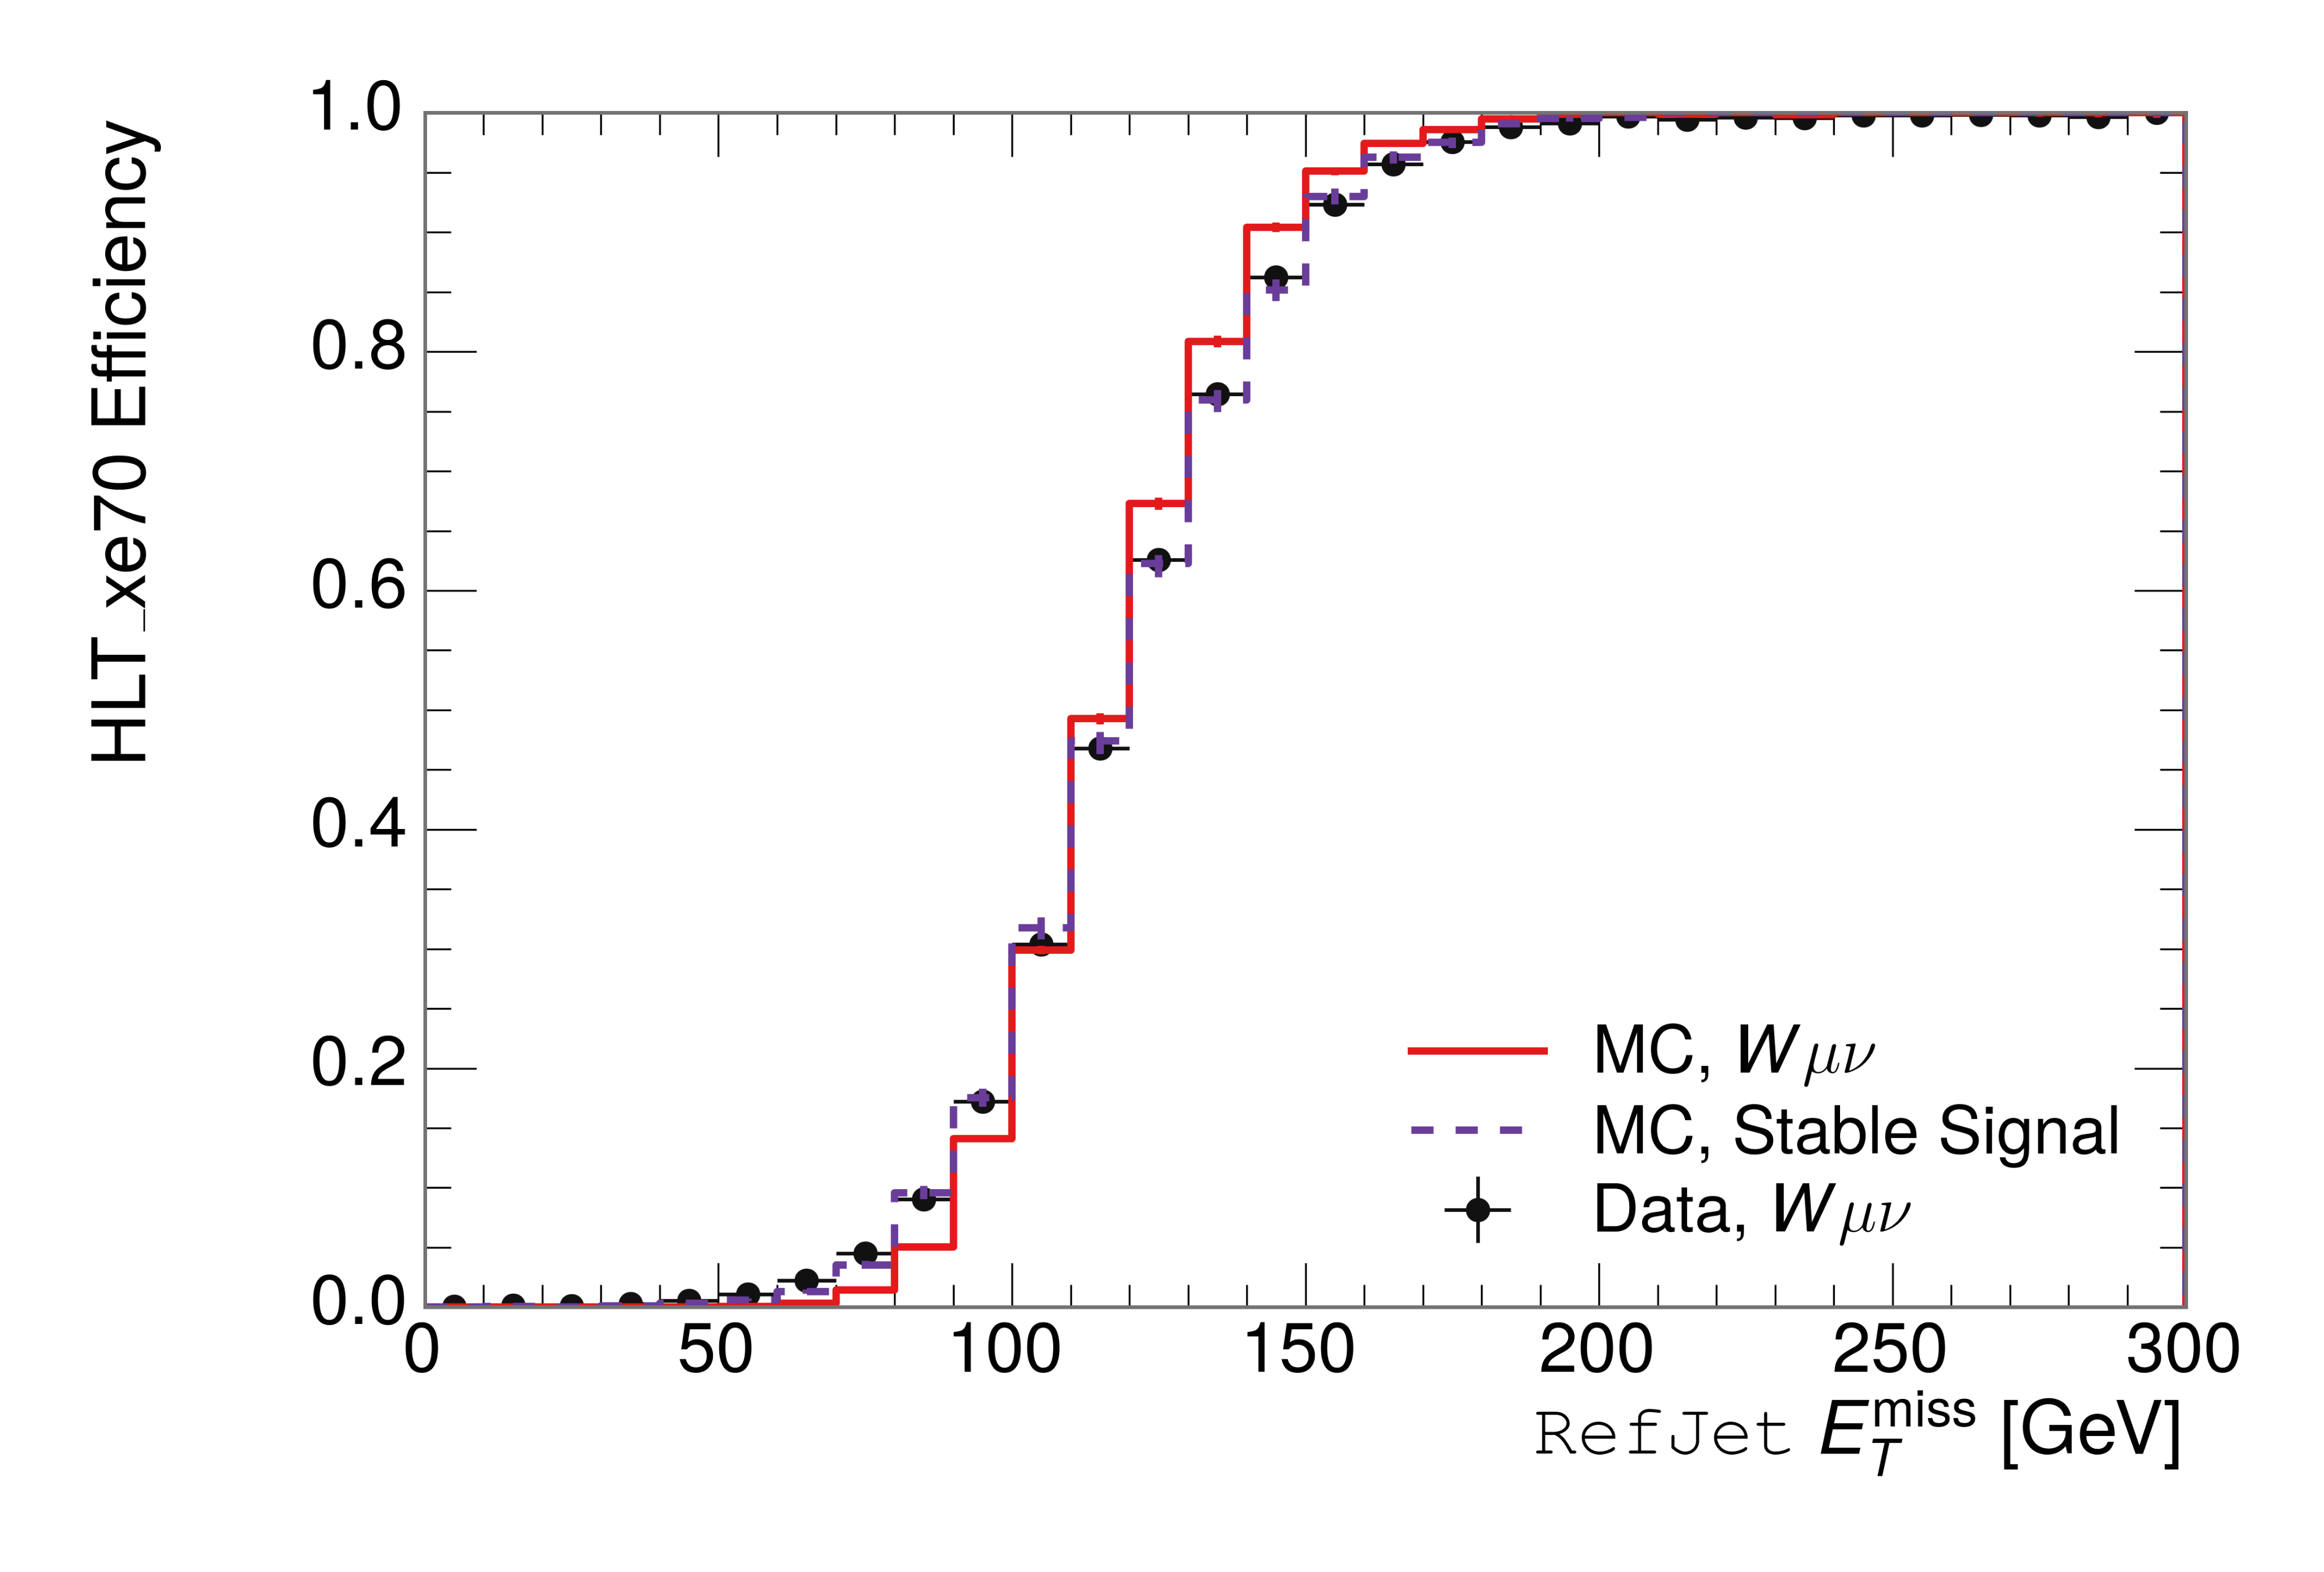
\includegraphics[width=\fullfig]{figures/hlt_xe70_calomet.png}
\caption{The trigger efficiency for the \texttt{HLT\_xe70} trigger requirement as a function of \calomet for simulated data events with a W boson selection. Simulated signal events and simulated W boson events are also included.}
\label{fig:trigger_turnon_calo}
\end{figure}

\subsection{Missing Transverse Momentum Scale}

Variations on the \ac{JES} enter into this analysis only in the requirement on \met, as variations on individual jets can alter the reconstructed \met in signal events. The effect of the measured \met is evaluated by varying the \met scale according to the one sigma variations on objects affecting event kinematics in simulated signal events. Missing energy is reconstructed from fully reconstructed objects so any systematic uncertainties affecting jets, muons, electrons, or the \met soft terms are included. The variations on these objects are taken from measurements in data using balance techniques as discussed in Section~\ref{sec:reco_jes}. The resulting difference in selection efficiency is expected to be small, because the jet variations only alter energies by a few percent. The only non-negligible contributions found using this method are itemized in Table~\ref{tab:met_syst_contributions} for an example signal sample (1200 GeV, \ac{VLL} R-Hadron), where the systematic is measured as the relative difference in the final signal efficiency after applying the associated variation through the CP tools. The only variations that are significant are the grouped jet systematic variations, which combine recommended jet systematic uncertainties into linearly independent variations. 

\begin{table}
  \begin{center}
  \begin{tabular}{lcc}
  \hline
  Systematic Variation & $-$[\%]& $+$[\%] \\
  \hline
  JET\_GroupedNP\_1 & $-0.7$ & 1.3\\
  JET\_GroupedNP\_2 & $-0.7$ & 1.2\\
  JET\_GroupedNP\_3 & $-0.5$ & 1.3\\
  \hline
  \end{tabular}
  \end{center}
  \caption{Example of the contributing systematic variations to the total systematic for the \met Scale, as measured in a 1200 GeV, \ac{VLL} R-Hadron signal sample.}
  \label{tab:met_syst_contributions}
\end{table}

As the peak of the reconstructed \met distribution in the signal is significantly above the current threshold for events which pass the trigger requirement, the effect of scale variation is expected to be small, which is consistent with the measured systematic error of approximately 2\%. Events which do not pass the trigger requirement usually fail because there are no ISR jets in the event to balance the $R$-hadrons' transverse momentum, so the reconstructed \met is low and therefore also expected to be not very sensitive to scale changes.

\subsection{Momentum Parametrization}
The uncertainty on the signal efficiency from track momentum is calculated using the sagitta bias for $q/P$. , the only systematic variation of tracking that effects track momentum.
The systematic is only important for tracks that are near the 150 \GeV momentum threshold, as the variation may push these tracks above or below the selection requirement.
Because the majority of \rhadron tracks are well above this value (Figure~\ref{fig:nm1_p}), the resulting uncertainty is expected to be small.
This uncertainty is propagated to the final selection efficiency by varying the track momentum by the measured one sigma variations from tracking measurements~\cite{ATL-PHYS-PUB-2015-051}, and the associated uncertainty is found to be negligible (0.3\%). 

\subsection{Ionization Requirement}
The $dE/dx$ distributions in data and simulated events have different most probable values, which is due in part to radiation effects in the detector that are not fully accounted for in the simulation. 
The difference does not affect the mass measurement used in this analysis, as independent calibrations are done in simulation and in data. 
However, it does affect the efficiency of the high $dE/dx$ selection requirement. 
To calculate the size of the effect on the signal efficiency, the $dE/dx$ distribution in signal simulation is scaled by a factor obtained from comparing the $dE/dx$ distribution of inclusive tracks in data and in simulation. 
The difference in efficiency for this sample with a scaled $dE/dx$ distribution, relative to the nominal case, is taken as a systematic uncertainty on signal efficiency.
The uncertainty is as large as 7\% for low masses and falls to a negligible effect for large masses. 

\subsection{Electron and Jet Rejection}
The systematic uncertainty on the electron rejection is measured by varying the EM fraction requirement significantly, from 0.95 to 0.9. 
This is found to have a less than 0.04\% effect on signal acceptance, on average, and so is completely negligible. Similarly, the uncertainty on jet rejection is measured by tightening the \ep requirement from 0.5 to 0.4. 
This is found to have no effect on signal acceptance, so again the systematic is again negligible.

\subsection{Muon Veto}
The signal region for \ac{LL} particles has a requirement that the candidate tracks are not identified as medium muons because the majority of \rhadrons in the lifetime range included in that region do not reach the muon spectrometers before they decay. 
However, the exponential tail of the \rhadron lifetime distribution results in some \rhadrons traversing the muon spectrometer. 
Even these \rhadrons can still fail the muon medium identification some of the time, because they may arrive late to the muon spectrometer as discussed in Section~\ref{sec:rh_interactions}.
The hits generated by a \rhadron will not be readout if it arrives 25 ns after the bunch crossing, causing it to fail the loose muon selection (Section~\ref{sec:muon_id}).
This can be seen in Figure~\ref{fig:muonVeto_eff}, which shows the efficiency of the muon veto as a function of $1/\beta$, for two simulated \ac{VLL} \rhadron samples.

\begin{figure}[hbtp]
\centering
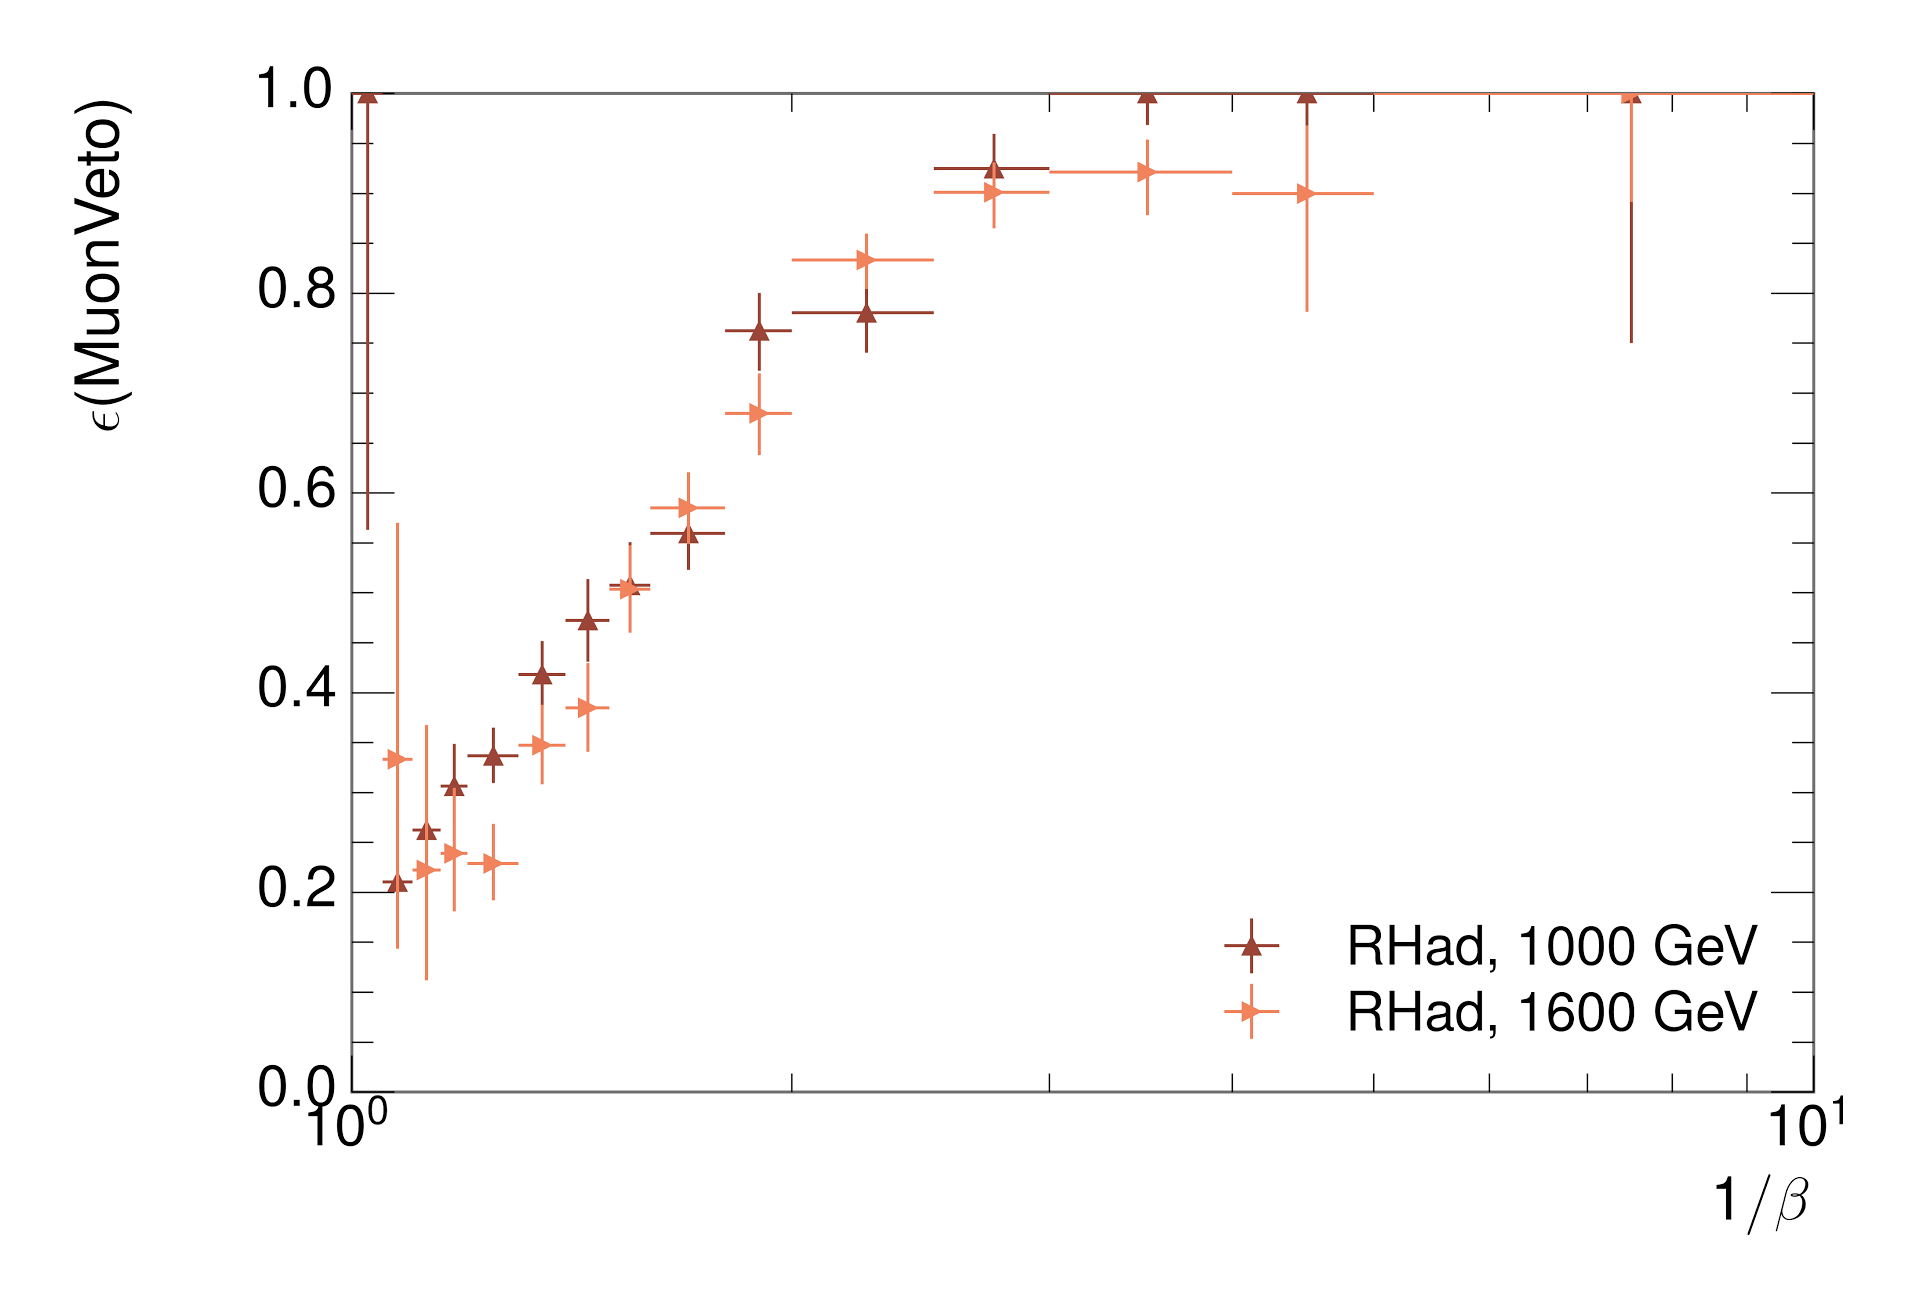
\includegraphics[width=\fullfig]{figures/veff_invbeta.png}
\caption{The efficiency of the muon veto for $R$-hadrons of two different masses, as a function of $\frac{1}{\beta}$ for simulated \rhadron tracks.}
\label{fig:muonVeto_eff}
\end{figure}

Thus, the efficiency of the muon veto depends on the timing resolution of the spectrometer, so an uncertainty is applied to the signal efficiency to cover differences in timing resolution between data and simulation. 
First, a sample of $Z\rightarrow\mu\mu$ events is selected in data in which one of the muons has a late arrival time measured in the \ac{MDT}. 
Then the reconstructed $\beta$ distribution is compared to the distribution in simulated $Z\rightarrow\mu\mu$ events; the difference between these two distributions reflects the difference in timing resolution between data and simulation.
To emulate this difference in simulated signal events, the magnitude of the difference is used to scale and shift the true $\beta$ distribution of \rhadrons in simulation. 
Signal events are then reweighted based on this varied $\beta$ distribution, and the difference in the efficiency of the muon veto selection is compared with the nominal and reweighted true $\beta$ distributions. 
The difference in muon veto efficiency is taken as a systematic uncertainty of the muon veto. 
 
The comparison of reconstructed $\beta$ between data and simulation is performed separately in the barrel, transition, and endcap regions of the spectrometer, and the reweighting of the true $\beta$ distribution in signal is done per region. 
The comparison of average reconstructed \ac{MDT} $\beta$ between data and simulation for the barrel region is shown in Figure~\ref{fig:mdt_beta} for $Z\rightarrow\mu\mu$ events.
As expected, The uncertainty is found to be negligible for $R$-hadrons with short lifetimes, and is only significant for lifetimes above 30 ns.

\begin{figure}[hbtp]
\centering
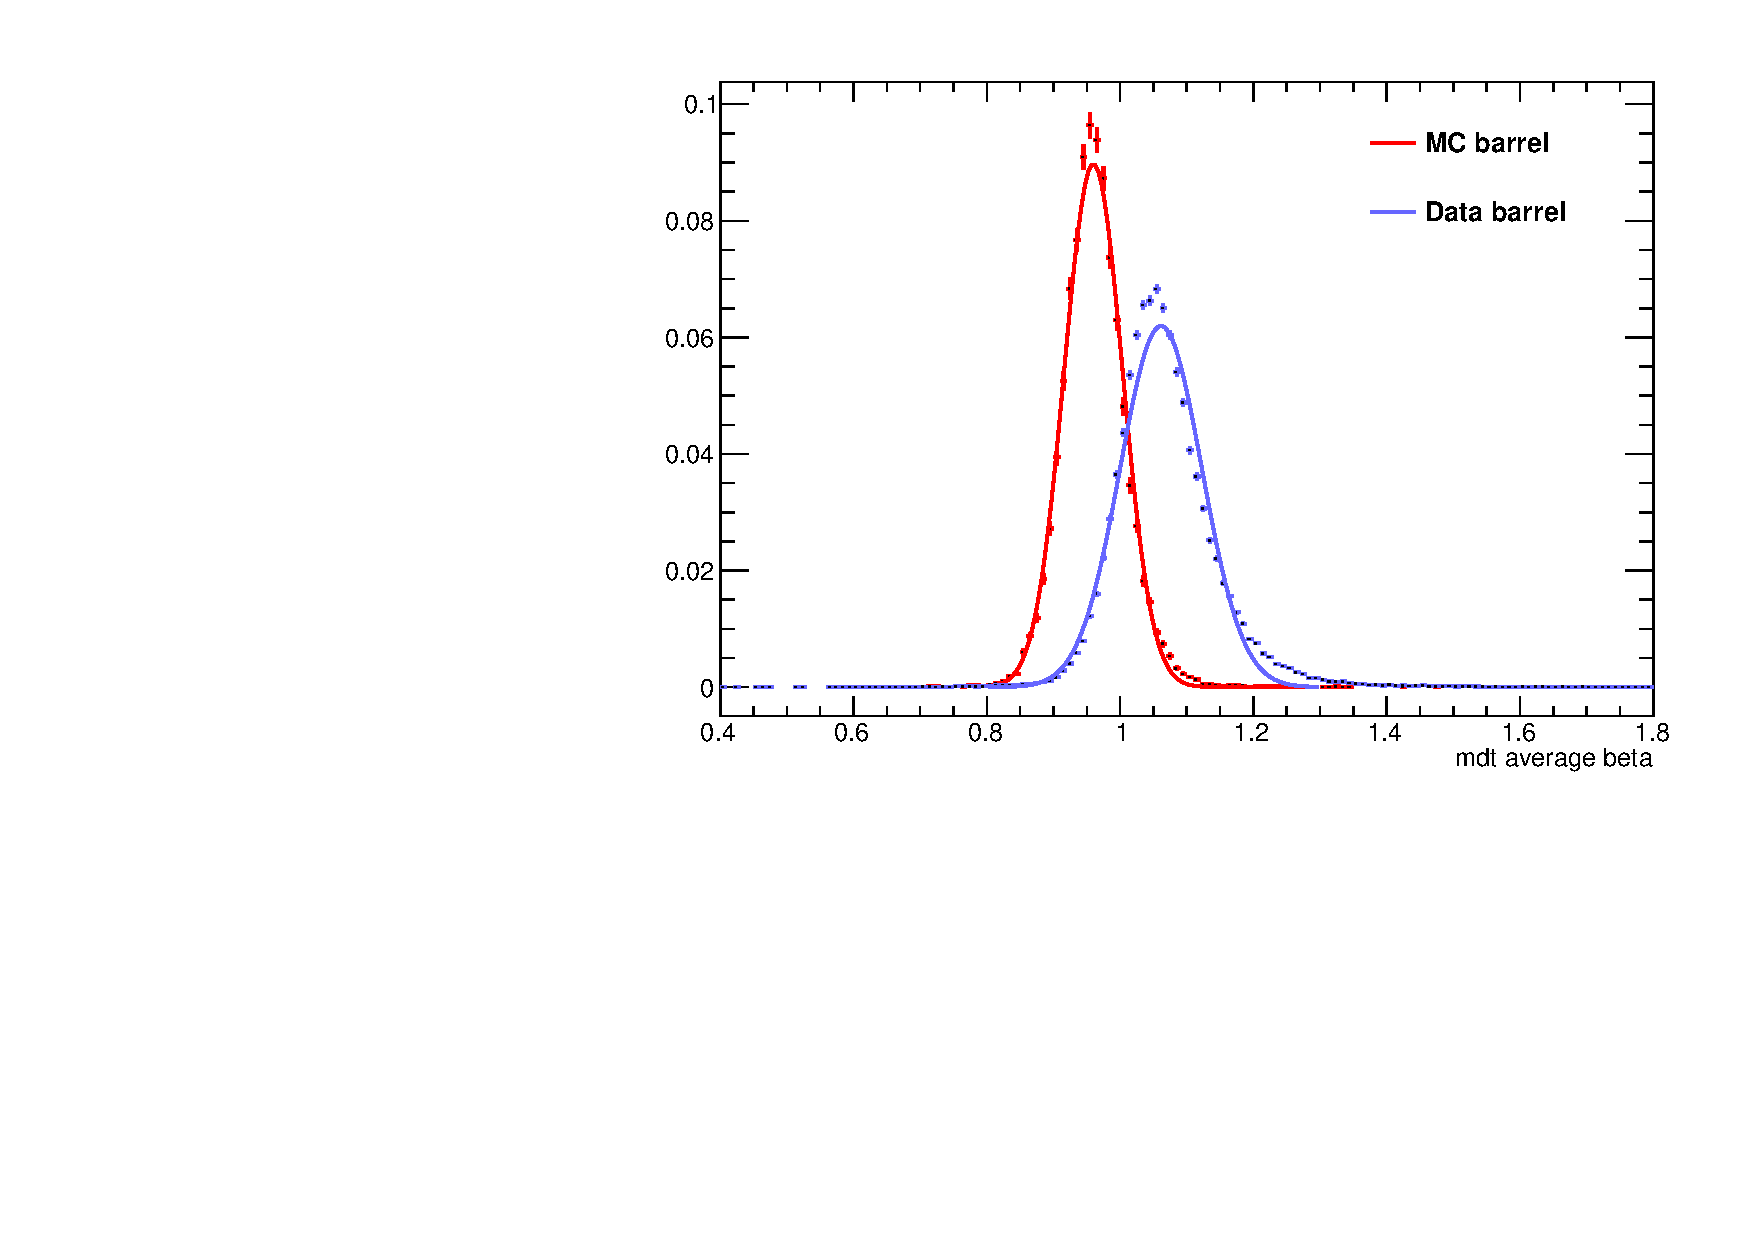
\includegraphics[width=\fullfig]{figures/beta_muonveto.pdf}
\caption{The average reconstructed MDT $\beta$ distribution for $Z\rightarrow\mu\mu$ events in which one of the muons has a late arrival time in the \acs*{MDT}, for both data and simulation. A gaussian fit is superimposed.}
\label{fig:mdt_beta}
\end{figure}

\subsection{Luminosity}
The luminosity uncertainty is provided by a luminosity measurement on ATLAS and was measured to be 5\% at the time of the publication of this analysis.
The uncertainty is estimated by comparing luminosity measurements using several independent luminometers~\cite{DAPR-2013-01}.

\subsection{Signal Cross Section}
As discussed in Section~\ref{sec:simulation_samples}, the signal cross sections are calculated at \ac{NLO} in the strong coupling constant with a resummation of soft-gluon emission at \ac{NLL}. 
The nominal predictions and the uncertainties for each mass point are taken from an envelope of cross-section predictions using different \ac{PDF} sets and factorization and renormalization scales~\cite{Kramer:2012bx}, as discussed in Section~\ref{sec:simulation_samples}.
The uncertainties on those cross sections range between 14\% and 28\% for \rhadrons in the range of 400 to 1800 \GeV~\cite{Mackeprang:2006gx, Mackeprang:2009ad}. 
The uncertainty increases with the mass.

% ----------------------------------------

